The astute reader may have noticed that the language \targetlang{}, and all the fragments and variations derived so far, exhibit a perfect symmetry for data and codata types and producers and consumers.
More precisely, producers of data (constructors) are perfectly symmetric to consumers of codata (destructors) and consumers of data (pattern matches) are perfectly symmetric to producers of codata (copattern matches).
We therefore can collapse the system along one of the axes shown in Figure \cref{fig:redundancy}.
Collapsing along the horizontal chirality axis means unifying producers and consumers, while collapsing along the vertical polarity axis means unifying data and codata types.
It seems more intuitive to collapse along the polarity axis, which still makes a producer and a consumer of the same type meet in a cut, resulting in a one-sided sequent calculus \cite{Girard1987}.

\begin{figure}[h!]
\tikzstyle{textonly}=[align=center, minimum width = 1.5cm, font=\small\sffamily]
\tikzstyle{box}=[textonly, rectangle, draw=black, minimum height = 1cm]
\tikzstyle{label}=[text=gray, align=center, font=\footnotesize\sffamily]

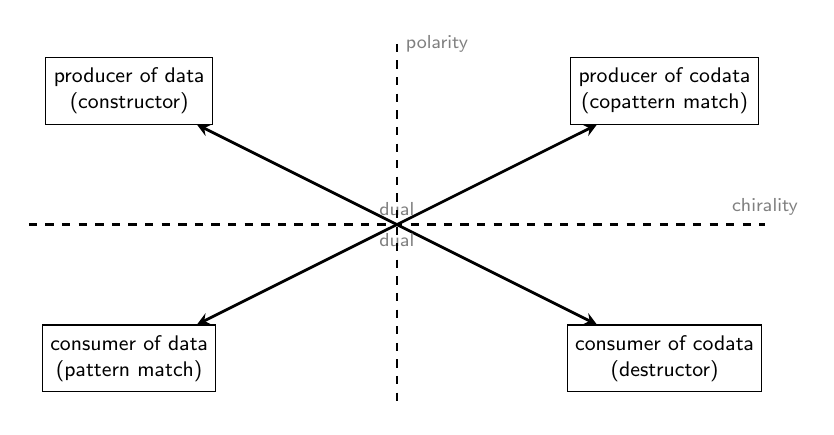
\begin{tikzpicture}[node distance=6cm, font=\footnotesize, scale=0.85, every node/.style={transform shape}]
  % Nodes
  \node (prddat) [box] at (0,0) {producer of data\\(constructor)};
  \node (cnsdat) [box] at (0,-4) {consumer of data\\(pattern match)};
  \node (prdcod) [box] at (8,0) {producer of codata\\(copattern match)};
  \node (cnscod) [box] at (8,-4) {consumer of codata\\(destructor)};

  % Arrows
  \draw [<->, >=stealth, line width = 1pt] (prddat) -- node[label, midway, above=0.1](dualtrivial){dual} (cnscod);
  \draw [<->, >=stealth, line width = 1pt] (cnsdat) -- node[label, midway, below=0.1](dualserious){dual} (prdcod);

  % Axes
  \draw [thick, dashed] (4,0.7) -- node[label, at start, right=0.1](pol){polarity} (4,-4.7);
  \draw [thick, dashed] (-1.5,-2) -- node[label, at end, above=0.1](chi){chirality} (9.5,-2);
\end{tikzpicture}

\noindent\caption{Redundancy in sequent calculus.}
\label{fig:redundancy}
\end{figure}

We use the following unified syntax for the resulting language called \machinelang, with a keyword-based syntax to make the rest of the paper more approachable to compiler engineers.

\begin{definition}[Syntax of AxCut]
    \[ 
      \begin{array}{r c l l}
        s & \coloneqq & \jump{f} \mid \substituteac{\Gamma \mapsto \Gamma}{s} \mid \done \mid \litac{n}{v}{s} \mid \opac{v, v}{v}{s} \mid \ifzac{v}{s}{s} & \emph{Statements}\\
        & \mid & \letac{v}{m\ \Gamma}{s} \mid \switch{v}{b} \mid \new{v}{\Gamma\ b}{s} \mid \invoke{v}{m} & \\
        b & \coloneqq & \bra{\overline{m\ \Gamma}} & \emph{Branches}\\
        v & \coloneqq & x \mid \alpha \mid j \mid \ldots & \emph{Variables}\\
        \tau & \coloneqq & \tyint \mid T & \emph{Types}\\
        \kappa & \coloneqq & \mathbf{sign} \mid \mathbf{prim} & \emph{Kinds}\\
        \Gamma & \coloneqq & \emptyset \mid \Gamma, v : \tau \mid \Gamma, v \cnt \tau \mid \Gamma, v \ext \tau & \emph{Typing Contexts} \\
        \delta & \coloneqq & \sig{T}{\overline{m\ \Gamma \Rightarrow s}} \mid \defi{f : \Gamma}{s} & \emph{Declarations}\\
        \Theta & \coloneqq & \overline{\delta} & \emph{Programs}\\
      \end{array}
    \]
\end{definition}

Here, $m$ is a unified notation for constructors $K$ and destructors $D$, and similarly $v$ stands for variables and covariables.
There are a few more differences to \targetsub.
We now use the $\jump{}$ construct instead of a call syntax for top-level definitions and we leave the arguments out in the syntax since they must constitute exactly the current environment.
Similarly, we leave the arguments out in the $\mathbf{invoke}$ statement where a producer $m$ is cut with a variable $v$ since the arguments of $m$ must constitute exactly the environment without $v$.
On the type level, we uniformly describe both data and codata types by signatures, without polarities, and call their unified kind $\mathbf{sign}$.
With this unification, a producer of a signature now represents a constructor or destructor and a consumer now represents a pattern match or copattern match.
We can choose to view a signature as a data type or a codata type.
We further introduce a separate typing judgment for primitive types, $\ext$, to distinguish them from producers of signatures.
Finally, we want to mention that we could make the terminal statement, the statements for integer literals and arithmetic operators and the statement for conditionals into special cases of a more general statement for external operations, $\extern{m(\overline{v_i})}{\overline{\Gamma_j \Rightarrow s_j}}$.
It is simple to extend the language with further instantiations of this general construct.

The translation from \targetsub{} to \machinelang{} mostly consists of renaming the statements to their unified counterparts.
Note how the perfectly symmetric statements of \targetsub{} are translated to exactly the same statement in \machinelang.
The most interesting part probably is the translation of type environments, where producers of data and consumers of codata in \targetsub{} are translated to the same judgment in \machinelang{} and likewise for consumers of data and producers of codata.

\begin{gather*}
  \begin{array}{rclrcl}
    \multicolumn{6}{c}{\collapse{\cdot} : \emph{Type}_{\targetsub{}} \rightarrow \emph{Type}_{\machinelang{}}}\\
    \collapse{\data{T}{\overline{K_i\ \Gamma_i}}}{} & \coloneq & \sig{T}{\overline{K_i\ \collapse{\Gamma_i}}} &
    \collapse{\Gamma, v : T}{} & \coloneq & \collapse{\Gamma}{}, v\ \collapse{: T} \\
    \collapse{\codata{T}{\overline{D_i\ \Gamma_i}}}{} & \coloneq & \sig{T}{\overline{D_i\ \collapse{\Gamma_i}}} &
    \collapse{: \tyint} & \coloneq & \ext \tyint \\
    \collapse{: T} & \coloneq & : T &
    \collapse{\cnt T} & \coloneq & \cnt T \\
    \multicolumn{3}{c}{\text{where } T : \mathbf{data}} &
    \multicolumn{3}{c}{\text{where } T : \mathbf{data}} \\
    \collapse{\cnt T} & \coloneq & : T &
    \collapse{: T} & \coloneq & \cnt T \\
    \multicolumn{3}{c}{\text{where } T : \mathbf{codata}} &
    \multicolumn{3}{c}{\text{where } T : \mathbf{codata}} \\
  \end{array}
  \\\\
  \begin{array}{rcl}
    \multicolumn{3}{c}{\collapse{\cdot} : \emph{Definition}_{\targetsub{}} \rightarrow \emph{Definition}_{\machinelang{}}}\\
    \collapse{\defi{f\ \Gamma}{s}} & \coloneq & \defi{f : \Gamma}{\collapse{s}} \\
  \end{array}
  \\\\
  \begin{array}{rclrcl}
    \multicolumn{6}{c}{\collapse{\cdot} : \emph{Statement}_{\targetsub{}} \rightarrow \emph{Statement}_{\machinelang{}}}\\
    \collapse{\cut{K\ \Gamma_0}{\tilde{\mu}x.s}} & \coloneq & \letac{x}{K\ \Gamma_0}{\collapse{s}} & \qquad
    \collapse{\cut{K\ \Gamma_0}{\alpha}} & \coloneq & \invoke{\alpha}{K} \\
    \collapse{\cut{\mu\alpha.s}{D\ \Gamma_0}} & \coloneq & \letac{\alpha}{D\ \Gamma_0}{\collapse{s}} &
    \collapse{\cut{x}{D\ \Gamma_0}} & \coloneq & \invoke{x}{D} \\
  \end{array}
  \\
  \begin{array}{rcl}
    \collapse{\cut{x}{\case{\overline{K_i\ \Gamma_i \Rightarrow s_i}}}} & \coloneq & \switch{x}{\bra{\overline{K_i\ \Gamma_i \Rightarrow \collapse{s_i}}}} \\
    \collapse{\cut{\cocase{\overline{D_i\ \Gamma_i \Rightarrow s_i}}}{\alpha}} & \coloneq & \switch{\alpha}{\bra{\overline{D_i\ \Gamma_i \Rightarrow \collapse{s_i}}}} \\
    \collapse{\cut{\mu\alpha.s}{\case{\overline{K_i\ \Gamma_i \Rightarrow s_i}}_{\Gamma_0}}} & \coloneq & \new{\alpha}{\Gamma_0 \bra{\overline{K_i\ \Gamma_i \Rightarrow \collapse{s_i}}}}{\collapse{s}} \\
    \collapse{\cut{\cocase{\overline{D_i\ \Gamma_i \Rightarrow s_i}}_{\Gamma_0}}{\tilde{\mu}x.s}} & \coloneq & \new{x}{\Gamma_0 \bra{\overline{D_i\ \Gamma_i \Rightarrow \collapse{s_i}}}}{\collapse{s}} \\
  \end{array}
  \\
  \begin{array}{rclrcl}
    \collapse{\cut{\lit{n}}{\tilde{\mu}x.s}} & \coloneq & \litac{n}{x}{\collapse{s}} &
    \collapse{\odot(x_1, x_2; \tilde{\mu}x.s)} & \coloneq & \opac{x_1, x_2}{x}{\collapse{s}} \\
    \collapse{\ifz{x}{s_1}{s_2}} & \coloneq & \ifzac{x}{\collapse{s_1}}{\collapse{s_2}} &
    \collapse{\done} & \coloneq & \done \\
    \collapse{\substitute{\Gamma \mapsto \Gamma^{\prime}}{s}} & \coloneq & \substituteac{\Gamma \mapsto \Gamma^{\prime}}{\collapse{s}} &
    \collapse{f\ \Gamma_0} & \coloneq & \jump{f} \\
  \end{array}
\end{gather*}


%%
%% Subsec: Typing Rules
%%
\subsection{Typing Rules}
\label{subsec:axcut:typing-rules}

For completeness, \cref{fig:axcut-rules} shows the full typing rules of \machinelang.

\begin{figure}[hbtp]
  \begin{minipage}{\textwidth}
  \vspace{1em}
  \judgementbox{Typing Statements}{$\Theta\mid\Gamma\vdash s$}

  \begin{minipage}{0.45\textwidth}
    \begin{prooftree}
      \AxiomC{$\Theta \mid \Gamma, v \ext \tyint \vdash s$}
      \RightLabel{\textsc{Lit}}
      \UnaryInfC{$\Theta \mid \Gamma \vdash \litac{n}{v}{s}$}
    \end{prooftree}
  \end{minipage}
  \hfill
  \begin{minipage}{0.45\textwidth}
    \begin{prooftree}
      \AxiomC{$v_1 \ext \tyint \in \Gamma$}
      \AxiomC{$v_2 \ext \tyint \in \Gamma$}
      \AxiomC{$\Theta \mid \Gamma, v \ext \tyint \vdash s$}
      \RightLabel{\textsc{Op}}
      \TrinaryInfC{$\Theta \mid \Gamma \vdash \opac{v_1, v_2}{v}{s}$}
    \end{prooftree}
  \end{minipage}
  \hfill
  \vspace{1em}

  \begin{minipage}{0.90\textwidth}
    \begin{prooftree}
      \AxiomC{$v \ext \tyint \in \Gamma$}
      \AxiomC{$\Theta \mid \Gamma \vdash s_1$}
      \AxiomC{$\Theta \mid \Gamma \vdash s_2$}
      \RightLabel{\textsc{Ifz}}
      \TrinaryInfC{$\Theta \mid \Gamma \vdash \ifzac{v}{s_1}{s_2}$}
    \end{prooftree}
  \end{minipage}
  \hfill
  \vspace{1em}

  \begin{minipage}{0.90\textwidth}
    \begin{prooftree}
      \AxiomC{$\sig{T}{{\ldots, m\ \Gamma_0, \ldots}} \in \Theta$}
      \AxiomC{$\Theta \mid \Gamma, v : T \vdash s$}
      \RightLabel{\textsc{Let}}
      \BinaryInfC{$\Theta \mid \Gamma, \Gamma_0 \vdash \letac{v}{m\ \Gamma_0}{s}$}
    \end{prooftree}
  \end{minipage}
  \hfill
  \vspace{1em}

  \begin{minipage}{0.90\textwidth}
    \begin{prooftree}
      \AxiomC{$\sig{T}{{\overline{m_i\ \Gamma_i}}} \in \Theta$}
      \AxiomC{$\overline{\Theta \mid \Gamma_i, \Gamma_0 \vdash s_i}$}
      \AxiomC{$\Theta \mid \Gamma, v \cnt T \vdash s$}
      \RightLabel{\textsc{New}}
      \TrinaryInfC{$\Theta \mid \Gamma, \Gamma_0 \vdash \new{v}{(\Gamma_0)\bra{\overline{m_i\ \Gamma_i \Rightarrow s_i}}}{s}$}
    \end{prooftree}
  \end{minipage}
  \hfill
  \vspace{1em}

  \begin{minipage}{0.45\textwidth}
    \begin{prooftree}
      \AxiomC{$\sig{T}{\overline{m_i\ \Gamma_i}} \in \Theta$}
      \AxiomC{$\overline{\Theta \mid \Gamma, \Gamma_i \vdash s_i}$}
      \RightLabel{\textsc{Switch}}
      \BinaryInfC{$\Theta \mid \Gamma, v : T \vdash \switch{v}{\bra{\overline{m_i \Gamma_i \Rightarrow s_i}}}$}
    \end{prooftree}
  \end{minipage}
  \hfill
  \begin{minipage}{0.45\textwidth}
    \begin{prooftree}
      \AxiomC{$\sig{T}{\ldots, m\ \Gamma, \ldots} \in \Theta$}
      \RightLabel{\textsc{Invoke}}
      \UnaryInfC{$\Theta \mid \Gamma, v \cnt T \vdash \invoke{v}{m}$}
    \end{prooftree}
  \end{minipage}
  \hfill
  \vspace{1em}

  \begin{minipage}{0.22\textwidth}
    \begin{prooftree}
      \AxiomC{\phantom{nothing}}
      \RightLabel{\textsc{Done}}
      \UnaryInfC{$\Theta \mid \Gamma \vdash \done$}
    \end{prooftree}
  \end{minipage}
  \hfill
  \begin{minipage}{0.43\textwidth}
    \begin{prooftree}
      \AxiomC{$\Theta \mid v'_1 :^{p} \tau, \ldots \vdash s$}
      \AxiomC{$v_1 :^{p} \tau \in \Gamma \ldots$}
      \RightLabel{\textsc{Substitute}}
      \BinaryInfC{$\Theta \mid \Gamma \vdash \substituteac{v'_1 \mapsto v_1, \ldots}{s}$}
    \end{prooftree}
  \end{minipage}
  \hfill
  \begin{minipage}{0.25\textwidth}
    \begin{prooftree}
      \AxiomC{$\mathbf{def}\ f\ \Gamma \in \Theta$}
      \RightLabel{\textsc{Jump}}
      \UnaryInfC{$\Theta \mid \Gamma \vdash \jump{f}$}
    \end{prooftree}
  \end{minipage}
  \hfill
  \vspace{1em}
\end{minipage}
\begin{minipage}{\textwidth}
  \vspace{1em}
  \judgementbox{Kinding Types}{$\Theta\vdash\tau:\kappa$}
  \begin{minipage}{0.4\textwidth}
    \begin{prooftree}
      \AxiomC{}
      \RightLabel{\textsc{PrimKind}}
      \UnaryInfC{$\Theta \vdash \tyint : \mathbf{prim}$}
    \end{prooftree}
  \end{minipage}
  \hfill
  \begin{minipage}{0.5\textwidth}
    \begin{prooftree}
      \AxiomC{$\sig{T}{\ldots} \in \Theta$}
      \RightLabel{\textsc{SignatureKind}}
      \UnaryInfC{$\Theta \vdash T : \mathbf{sign}$}
    \end{prooftree}
  \end{minipage}
  \vspace{1em}
\end{minipage}
\begin{minipage}{\textwidth}
  \vspace{1em}
  \judgementbox{Well-formed Programs}{$\vdash \wellformed{\Theta}$}
  \begin{minipage}{0.2\textwidth}
    \begin{prooftree}
      \AxiomC{}
      \RightLabel{\textsc{Wf-Empty}}
      \UnaryInfC{$\vdash \wellformed{\nil}$}
    \end{prooftree}
  \end{minipage}
  \hfill
  \begin{minipage}{0.75\textwidth}
    \begin{prooftree}
      \AxiomC{$\vdash \wellformed{\Theta}$}
      \AxiomC{$\overline{\Theta,\sig{T}{\dots}\vdash\goodctx{\Gamma_i}}$}
      \AxiomC{$\overline{ \Gamma_i \vdash \tau_i:\kappa}$}
      \RightLabel{\textsc{Wf-Signature}}
      \TrinaryInfC{$\vdash \wellformed{\Theta,\sig{T}{ \overline{m_i\ \Gamma_i}}}$}
    \end{prooftree}
  \end{minipage}
  \hfill
  \vspace{1em}

  \begin{minipage}{0.90\textwidth}
    \begin{prooftree}
      \AxiomC{$\vdash \wellformed{\Theta}$}
      \AxiomC{$\Theta, \defi{f : \Gamma}{s} \mid\Gamma \vdash s$}
      \RightLabel{\textsc{Wf-Def}}
      \BinaryInfC{$\vdash \wellformed{\Theta,\defi{f : \Gamma}{s}}$}
    \end{prooftree}
  \end{minipage}
  \hfill
  \vspace{1em}
\end{minipage}
\begin{minipage}{\textwidth}
  \vspace{1em}
  \judgementbox{Well-formed Contexts}{$\Theta\vdash \goodctx{\Gamma}$}
  \begin{minipage}{0.45\textwidth}
    \begin{prooftree}
      \AxiomC{\phantom{$x\in\nil$}}
      \RightLabel{\textsc{Ctx}$_1$}
      \UnaryInfC{$\Theta\vdash\goodctx{\nil}$}
    \end{prooftree}
  \end{minipage}
  \hfill
  \vspace{1em}
  \begin{minipage}{0.45\textwidth}
    \begin{prooftree}
      \AxiomC{$\Theta\vdash\goodctx{\Gamma} \quad v\notin\Gamma \quad \Theta\vdash\tau:\kappa$}
      \RightLabel{\textsc{Ctx}$_2$}
      \UnaryInfC{$\Theta\vdash\goodctx{\Gamma,v:\tau}$}
    \end{prooftree}
  \end{minipage}
  \hfill
  \vspace{1em}
  \begin{minipage}{0.45\textwidth}
    \begin{prooftree}
      \AxiomC{$\Theta\vdash\goodctx{\Gamma} \quad v\notin\Gamma \quad \Theta\vdash\tau:\kappa$}
      \RightLabel{\textsc{Ctx}$_3$}
      \UnaryInfC{$\Theta\vdash \goodctx{\Gamma,v\cnt\tau}$}
    \end{prooftree}
  \end{minipage}
  \hfill
  \vspace{1em}
  \begin{minipage}{0.45\textwidth}
    \begin{prooftree}
      \AxiomC{$\Theta\vdash\goodctx{\Gamma} \quad v\notin\Gamma \quad \Theta\vdash\tau:\kappa$}
      \RightLabel{\textsc{Ctx}$_4$}
      \UnaryInfC{$\Theta\vdash \goodctx{\Gamma,v\ext\tau}$}
    \end{prooftree}
  \end{minipage}
  \hfill
  \vspace{1em}
\end{minipage}
\caption{Typing rules for \machinelang{}}
\label{fig:axcut-rules}
\end{figure}
